\documentclass{article}

\usepackage[final]{neurips_2022}
%\usepackage[UTF8]{ctex}

\usepackage[utf8]{inputenc}
\usepackage[T1]{fontenc}
\usepackage{hyperref}
\usepackage{url}
\usepackage{booktabs}
\usepackage{amsfonts}
\usepackage{nicefrac}
\usepackage{float}
\usepackage{amsmath}
\usepackage{amssymb}
\usepackage{amsthm}
\usepackage{algorithm}
\usepackage{algpseudocode}
\usepackage{microtype}
\usepackage{xcolor}
\usepackage{bm}
\usepackage{graphicx}
\usepackage{subfigure}
\usepackage{listings}
\usepackage{quantikz}
\usepackage{caption}
\usepackage{tikz}
\usetikzlibrary{trees}
\hypersetup{
  colorlinks=true,
  linkbordercolor=white,
}
\newtheorem{definition}{Definition}[section]
\newtheorem{theorem}{Theorem}[section]
\renewcommand{\algorithmicrequire}{\textbf{Input:}}
\renewcommand{\algorithmicensure}{\textbf{Output:}}

\title{Explicit Quantum Circuits for Block Encodings of Sparse Matrices: A Review and Exploration}

\author{%
  \large Zibo Ren \\
  \large \texttt{2200010626}
  \And
  \large Zixuan Yuan \\
  \large \texttt{2200010825}
}

\begin{document}

\maketitle

\begin{abstract}

  Efficiently constructing quantum circuits for block encodings of matrices is crucial for leveraging quantum linear algebra algorithms, which promise significant speedups for many computational problems.
  A block encoding is a technique where a matrix of interest is embedded within a larger unitary matrix, making it amenable to quantum computation.
  The realization of quantum advantage, however, heavily relies on the effective construction of these block encoding circuits, a task that presents considerable challenges, even when dealing with well-structured sparse matrices.
  This report reviews the work by Camps et al. \cite{EQC} on explicit circuit constructions for block encodings of certain well-structured sparse matrices.
  We delve into their proposed strategies, analyze their numerical demonstrations and reproduce their experiments.
  Furthermore, we explore potential avenues for original contributions and future research directions stemming from this work.
  We also provide implementations of the quantum circuits discussed in this paper in Python.

\end{abstract}

\section{Introduction}

Quantum linear algebra algorithms have emerged as a promising avenue to achieve exponential speedups over classical counterparts in solving fundamental computational problems such as solving linear systems, eigenvalue decomposition, and singular value transformation \cite{EQC}. At the heart of these algorithms lies the technique of \emph{block encoding}, which enables the embedding of non-unitary matrices into larger unitary matrices\textemdash a prerequisite for quantum computation. Formally, an $(\alpha, m, \varepsilon)$-block-encoding of a matrix $A \in \mathbb{C}^{N \times N}$ involves constructing an $(m+n)$-qubit unitary $U_A$ such that
\begin{equation}
  \|A - \alpha(\bra{0^m} \otimes I_N)U_A(\ket{0^m} \otimes I_N)\|_2 \leq \varepsilon
\end{equation}
where $N=2^n$. However, despite theoretical guarantees of algorithmic efficiency, practical implementations of block encodings remain challenging, particularly for structured sparse matrices\textemdash a critical class of inputs for applications in graph theory, differential equations, and machine learning.

Prior work on block encoding primarily focused on abstract oracle-based constructions, leaving explicit circuit designs largely unexplored. For instance, while quantum singular value transformation (QSVT) \cite{Gilyen2019} theoretically enables polynomial transformations of matrices via block encodings, its practical utility hinges on the explicit construction of quantum circuits for structured matrices. Camps et al. \cite{EQC} recently addressed this gap by introducing a systematic framework for constructing efficient quantum circuits for $s$-sparse matrices, which are matrices with at most $s$ nonzeros per column. Their approach decomposes the block encoding unitary $U_A$ into two components: (1) an oracle circuit $O_C$ that encodes the sparsity pattern of $A$, and (2) an oracle circuit $O_A$ that encodes the numerical values of nonzero entries. This explicit decomposition bridges the gap between theoretical algorithms and hardware-realizable implementations.

The significance of this work is twofold. First, for scaled $s$-sparse matrices $A/s$, the authors demonstrate circuits with gate complexity $\text{poly}(n)$, where $n$ is the qubit count, by leveraging controlled rotations and shift operators (e.g., implementing the mapping $\ket{j} \mapsto \ket{\text{mod}(j \pm 1, N)}$ for cyclic graph adjacency matrices) \cite{EQC}. Second, they extend their framework to symmetric stochastic matrices, enabling direct block encodings of Chebyshev polynomials $T_k(P)$ for quantum walks\textemdash a task previously hindered by scaling factors $1/s$ that degraded algorithmic efficiency. For example, their explicit construction of a quantum circuit for the block encoding of a $8 \times 8$ circulant matrix achieves optimal depth by combining Hadamard gates and controlled-$R$ shifts (Fig. 7 in \cite{EQC}).

This review synthesizes the key contributions of Camps et al. \cite{EQC}, including their general strategy for sparse matrix block encoding, numerical demonstrations using the QCLAB toolbox in MATLAB, and connections to quantum walk algorithms. We provide Python implementations of their circuits for reproducibility. By analyzing both theoretical and practical aspects, this report aims to illuminate pathways for advancing quantum linear algebra algorithms in real-world applications.

All quantum circuits figures in this paper are generated using the Python library \texttt{qiskit}. Our code is available at \url{https://github.com/0Ishtar0/QASC}.

\section{Related Works}

\label{sec:related_works}

Theoretical Foundations of Block Encoding is concerned with establishing mathematical frameworks for embedding matrices into unitary operations. Pioneering work by Low and Chuang\cite{low2017optimal}
introduced methods to encode singular values into quantum amplitudes, while Chakraborty et al.\cite{chakraborty2018power}
extended this to arbitrary matrices, deriving sparsity-dependent complexity bounds. These studies focus on asymptotic guarantees rather than explicit circuit implementations, leaving practical deployment challenges unaddressed.

Circuit-Oriented Optimizations for Structured Matrices is focused on leveraging matrix-specific properties to design efficient quantum circuits.
Berry et al \cite{berry2015hamiltonian} suggested that such a quantum circuit can
be constructed in theory for certain sparse matrices, the proposed construction relies on the availability of “oracles" that
can efficiently encode both the nonzero structure of A and numerical values of the nonzero matrix elements, but getting such oracles is not trivial.
The original paper exploit sparsity patterns to minimize gate counts by introducing reusable circuit components and integrating them with the QCLAB framework
, enabling verifiable implementations for structured sparse matrices.

Approximate Methods for NISQ Devices is driven by the need to adapt block encodings to near-term hardware constraints. Techniques like FABLE \cite{camps2022fable}
trade precision for reduced circuit depth through classical preprocessing and parameterized quantum ansätze. While effective for noisy environments, these approximations degrade performance in high-accuracy applications such as quantum chemistry
, where exact block encodings remain indispensable.

Algorithmic Applications of Block Encodings is centered on deploying block-encoded matrices in critical quantum algorithms. QSVT-based solvers \cite{Gilyen2019}for differential equations
and machine learning models rely on this framework, which the explicit circuits directly accelerate by reducing the overhead of compiling abstract encodings into physical gates.

Quantum algorithm simulation aims to model the behavior of quantum algorithms using classical computers.
QCLAB \cite{keip2025qclab} is an object-oriented MATLAB toolbox that provides visualization and simulation capabilities for quantum circuits, enabling researchers to verify and optimize the implementation of quantum algorithms .
Correspondingly, Qiskit\cite{wille2019ibm} is a Python-based software development kit (SDK) that offers similar functionalities, making the design, simulation, and execution of quantum circuits more flexible and accessible .
Through these tools, researchers can test and validate their algorithms on actual quantum hardware, thereby advancing the practical applications of quantum computing.

\section{Preliminary}\label{sec:preliminary}
In this section, we introduce the necessary mathematical and quantum computing concepts that underpin the construction of block encodings for sparse matrices.
As the basis for quantum algorithms, we use the $\bra{\cdot}$ and $\ket{\cdot}$ notation to denote the complex conjugate and quantum state vector, respectively. In particular, we use the notation $\ket{n}$ to represent the n-th basis in a $2^k$-dimensional Hilbert space, where $k$ is the number of qubits.

We present the notations for several common quantum gates, for example, the Hadamard gate $H$, the Pauli gates $X$, $Y$, and $Z$, defined as follows:
\begin{equation}
  H = \frac{1}{\sqrt{2}}
  \begin{bmatrix}
    1 & 1  \\
    1 & -1
  \end{bmatrix}, \qquad
  X =
  \begin{bmatrix}
    0 & 1 \\
    1 & 0
  \end{bmatrix}, \qquad
  Y =
  \begin{bmatrix}
    0 & -i \\
    i & 0
  \end{bmatrix}, \qquad
  Z =
  \begin{bmatrix}
    1 & 0  \\
    0 & -1
  \end{bmatrix}\label{eq:equation}
\end{equation}
Moreover, rotation matrices about the Pauli-$Y$ axis are crucial components in constructing block encoding circuits and can be expressed as
\begin{equation}
  R_y(\theta) :=
  \begin{bmatrix}
    \cos\left(\frac{\theta}{2}\right) & -\sin\left(\frac{\theta}{2}\right) \\
    \sin\left(\frac{\theta}{2}\right) & \cos\left(\frac{\theta}{2}\right)
  \end{bmatrix}
  = e^{-i \frac{\theta}{2} Y}, \tag{2.2} \label{eq:RY}
\end{equation}
where $\theta$ denotes the rotation angle and the unitary $Y$ is defined in Eq.~\eqref{eq:equation}. The matrices in Eqs.~\eqref{eq:equation} and \eqref{eq:RY} are $2 \times 2$ unitary operators that serve as fundamental single-qubit quantum gates.

Additionally,a significant category of quantum gates is the controlled gates, where one or more qubits function as control elements for an operation.
Graphically, control operations are depicted using a vertical line connecting the control qubit(s) to the target gate, which may be a single gate or a subcircuit block, such as a controlled-NOT (CNOT) gate(Fig.~\ref{fig:controlled-gates}).
A filled circle on the control line signifies that the target operation is executed when the control qubit is in state $\ket{1}$ , whereas an unfilled circle indicates execution when the control qubit is in state $\ket{0}$ .
\begin{figure}[htbp]
  \centering
  \subfigure[$\ket{0}$ controlled]{            \centering\label{fig:0-controlled-gates}
    \begin{quantikz}
      \lstick{$q_0$} & \octrl{1} & \qw \\
      \lstick{$q_1$} & \targ{} & \qw
    \end{quantikz}
    \hspace{0.5cm}
    $=$
    \hspace{0.5cm}
    $
    \begin{bmatrix}
      0 & 1 & 0 & 0 \\
      1 & 0 & 0 & 0 \\
      0 & 0 & 1 & 0 \\
      0 & 0 & 0 & 1
    \end{bmatrix}$
  }
  \hspace{1cm}
  \subfigure[$\ket{1}$ controlled]{            \centering\label{fig:1-controlled-gates}
    \centering
    \begin{quantikz}
      \lstick{$q_0$} & \ctrl{1} & \qw \\
      \lstick{$q_1$} & \targ{} & \qw
    \end{quantikz}
    \hspace{0.5cm}
    $=$
    \hspace{0.5cm}
    $
    \begin{bmatrix}
      1 & 0 & 0 & 0 \\
      0 & 1 & 0 & 0 \\
      0 & 0 & 0 & 1 \\
      0 & 0 & 1 & 0
    \end{bmatrix}$
  }
  \caption{Controlled-NOT gates with $\ket{0}$ and $\ket{1}$ controls and their matrix representations.}\label{fig:controlled-gates}
\end{figure}

Mathematically, the controlled gates depicted in Fig.~\ref{fig:controlled-gates} correspond to the expressions
\begin{equation}
  E_0 \otimes X + (I - E_0) \otimes I \quad \text{and} \quad E_1 \otimes X + (I - E_1) \otimes I
\end{equation}
where the orthogonal projection operators
\begin{equation}
  E_0 = e_0 e_0^T = \ket{0} \bra{0}, \qquad E_1 = e_1 e_1^T = \ket{1}\bra{1}.
\end{equation}
These operators act as control elements.
Specifically, the NOT ($X$) operation is applied to qubit $q_1$ (Fig.~\ref{fig:0-controlled-gates}) only when the input to qubit $q_0$ is $\ket{0}$. Analogously, the NOT operation is triggered for qubit $q_1$ (Fig.~\ref{fig:1-controlled-gates}) if the input to $q_0$ is $\ket{1}$.
This formulation can be extended to describe multi-qubit controlled-NOT gates.

Throughout this paper, we use the python library \texttt{qiskit} \cite{wille2019ibm} to implement and draw quantum circuits for bolck-encoding sparse matrices.
This library provides tools to compute the unitary representation of a quantum circuit, which is essential for analyzing the circuit's theoretical significance.
For example, the quantum circuit in Fig.~\ref{fig:circuit1} can be implemented in \texttt{qiskit} as follows:

    \begin{lstlisting}[language=Python, label={lst:ghz-circuit}]
    qc = QuantumCircuit(3, 3)
    qc.h(0)
    qc.cx(0, 1)
    qc.cx(0, 2)
    qc.measure([0, 1, 2], [0, 1, 2])
    \end{lstlisting}

This circuit represents a three-qubit GHZ state, which is a fundamental quantum state used in various quantum algorithms and protocols.
To generate a GHZ state, we apply a Hadamard gate on the first qubit to create superposition, followed by two CNOT gates to entangle it with the second and third qubits.
This gate can be represented as $\ket{GHZ} = (\ket{000}+\ket{111})/\sqrt{2}$.

\begin{figure}[htbp]
  \centering
  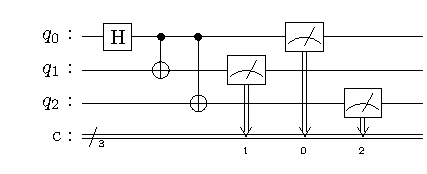
\includegraphics{pdf/example}
  \caption{
    GHZ State
  }
  \label{fig:circuit1}
\end{figure}

\section{Efficient Block Encoding of Sparse Matrices}\label{sec:block_encoding}
\begin{definition}[Block encoding]
  \label{def:block_encoding}
  Given an $n$-qubit matrix $A$ ($N = 2^n$), if we can find $\alpha, \epsilon \in \mathbb{R}_+$, and an $(m + n)$-qubit unitary matrix $U_A$ so that
  \begin{equation}
    \left\| A - \alpha \left( \bra{0^m} \otimes I_N \right) U_A \left( \ket{0^m} \otimes I_N \right) \right\|_2 \leq \epsilon,\label{eq:equation2}
  \end{equation}
  then $U_A$ is called an $(\alpha, m, \epsilon)$-block-encoding of $A$. In particular, when the block encoding is exact with $\epsilon = 0$, $U_A$ is called an $(\alpha, m)$-block-encoding of $A$.
\end{definition}

For a simple illustration, consider encoding a scalar $a \in \mathbb{R}$ such that $|a| \leq 1$. This can be viewed as a $1 \times 1$ matrix $A=[a]$, so $N=1$ (requiring $n=0$ system qubits). We can construct a $(1, 1, 0)$-block encoding using one ancilla qubit ($m=1$). The unitary $U_A$ is the single-qubit rotation gate $R_Y(2 \arccos a)$ applied to the ancilla qubit:
\begin{equation}
  U_A = R_Y(2 \arccos a) =
  \begin{bmatrix}
    \cos(\arccos a) & -\sin(\arccos a) \\ \sin(\arccos a) & \cos(\arccos a)
  \end{bmatrix} =
  \begin{bmatrix}
    a & -\sqrt{1-a^2} \\ \sqrt{1-a^2} & a
  \end{bmatrix}.\label{eq:equation3}
\end{equation}
According to Definition~\ref{def:block_encoding}, with $\alpha=1$ and $\epsilon=0$:
$$ \left( \bra{0} \otimes I_0 \right) U_A \left( \ket{0} \otimes I_0 \right) = \bra{0} U_A \ket{0}. $$
Since $I_0$ (the identity for a 0-qubit system) is a scalar 1, this expression selects the top-left element of $U_A$, which is $a$. Thus, $R_Y(2 \arccos a)$ is a $(1,1,0)$-block encoding of $A=[a]$. The quantum circuit for $U_A$ is shown in Fig.~\ref{fig:scalar_block_encode}.

\begin{figure}[H]
  \centering
  \begin{quantikz}
    \lstick{$\ket{0}_{\text{ancilla}}$} & \gate{R_Y(2\arccos a)} & \qw
  \end{quantikz}
  \caption{Quantum circuit for a $(1,1,0)$-block encoding of a scalar $a$. The single qubit shown is the ancilla qubit. The operation $R_Y(2\arccos a)$ embeds $a$ into the top-left element of its matrix representation.}
  \label{fig:scalar_block_encode}
\end{figure}

This basic example highlights how a matrix (even a scalar) can be embedded as a block within a larger unitary operation, which is a fundamental concept for many quantum algorithms.

In this section, we consider the block encoding of structured and s-sparse matrices, which are matrices with at most $s$ nonzero entries both per column and per row. Without loss of generality, we assume that $s = 2^m\ll N$for some integer $m \ll n$.
If $s$ is not a power of 2, we can treat the matrix as a $2^m$-sparse matrix by counting zeros as non-zeros, which does not affect the block encoding. The following theorem provides a general framework for constructing block encodings of $s$-sparse matrices if we have some oracles.

\begin{theorem}
  \label{thm:main_result}
  Let $c(j, \ell)$ be a function that gives the row index of the $\ell$th (among a list of $s$) non-zero matrix elements in the $j$th column of an $s$-sparse matrix $A \in \mathbb{C}^{N \times N}$ with $N = 2^n$, where $s = 2^m$. If there exists a unitary $O_c$ such that
  \begin{equation}
    O_c \ket{\ell} \ket{j} = \ket{\ell} \ket{c(j, \ell)},\label{eq:equation4}
  \end{equation}
  and a unitary $O_A$ such that
  \begin{equation}
    O_A \ket{0} \ket{\ell} \ket{j} = \left( A_{c(j, \ell), j} \ket{0} + \sqrt{1 - |A_{c(j, \ell), j}|^2} \ket{1} \right) \ket{\ell} \ket{j},\label{eq:equation5}
  \end{equation}
  then
  \begin{equation}
    U_A = (I_2 \otimes D_s \otimes I_N)(I_2 \otimes O_c) \, O_A \, (I_2 \otimes D_s \otimes I_N),\label{eq:equation6}
  \end{equation}
  block encodes $A/s$. Here $D_s$ is called a diffusion operator and is defined as
  \begin{equation}
    D_s \equiv \underbrace{H \otimes H \otimes \cdots \otimes H}_{m},\label{eq:equation7}
  \end{equation}
\end{theorem}

\begin{proof}
  The proof is straightforward. We will apply the gates to the input state $\ket{0^{m+1}}\ket{j}$ step by step.
  First, we apply the diffusion operator $D_s$ to the first $m$ qubits, which transforms $\ket{0^m}$ into a uniform superposition over all $s$ states:
  \begin{equation}
    D_s \ket{0^m} = \frac{1}{\sqrt{s}} \sum_{\ell=0}^{s-1} \ket{\ell}.\label{eq:equation8}
  \end{equation}
  Next, we apply the oracle $O_A$ and $O_c$ to $\ket{0}\ket{m}\ket{j}$:
  \begin{equation}
    \begin{aligned}
      \ket{0} \ket{0^m} \ket{j}
      &\xrightarrow{D_s} \frac{1}{\sqrt{s}} \sum_{\ell \in [s]} \ket{0} \ket{\ell} \ket{j} \\
      &\xrightarrow{O_A} \frac{1}{\sqrt{s}} \sum_{\ell \in [s]} \left( A_{c(j, \ell), j} \ket{0} + \sqrt{1 - |A_{c(j, \ell), j}|^2} \ket{1} \right) \ket{\ell} \ket{j} \\
      &\xrightarrow{O_c} \frac{1}{\sqrt{s}} \sum_{\ell \in [s]} \left( A_{c(j, \ell), j} \ket{0} + \sqrt{1 - |A_{c(j, \ell), j}|^2} \ket{1} \right) \ket{\ell} \ket{c(j, \ell)}.
    \end{aligned}\label{eq:equation9}
  \end{equation}

  Finally, we reverse the quantum circuit by considering the last quantum gate $D_s$ and applying its transpose to another input quantum state $\ket{0}\ket{0^m}\ket{i}$:

  \begin{equation}
    \ket{0} \ket{0^m} \ket{i}
    \xrightarrow{D_s} \frac{1}{\sqrt{s}} \sum_{\ell \in [s]} \ket{0} \ket{\ell} \ket{i}\label{eq:equation10}.
  \end{equation}

  Combining Eqs.~\eqref{eq:equation9} and \eqref{eq:equation10}, we can calculate the inner product of two input states $\ket{0^m}\ket{j}$ and $\ket{0^m}\ket{i}$:

  \begin{equation}
    \bra{0} \bra{0^m} \bra{i} U_A \ket{0} \ket{0^m} \ket{j}
    = \frac{1}{s} \sum_{\ell} A_{c(j, \ell), j} \delta_{i, c(j, \ell)}
    = \frac{1}{s} A_{ij}.\label{eq:equation11}
  \end{equation}

  Since the $\ket{i}$ form an orthonormal basis, by the linearity of matrix-vector multiplication, it follows that the quantum circuit $U_A$ in the theorem provides a $(1/s,m+1,0)$ -block-encoding of $A$.

\end{proof}

The full quantum circuit is shown in Fig.~(\ref{fig:circuit2}).
While one could potentially manually design a collection of controlled operations to explicitly enforce Eqs.~\eqref{eq:equation5} and \eqref{eq:equation6} for particular values of $j$ and $\ell$, such an approach would result in an inefficient circuit architecture.
This is due to the fact that the total number of quantum gates required would scale as $\mathcal{O}(N)$, which grows exponentially with $n$.
Similarly, alternative naive implementations like the method introduced by Camps et al.~\cite{camps2022fable} could still necessitate $\mathcal{O}(N)$ operations.
The original paper developed a quantum circuit with polynomial gate complexity---\emph{i.e.}, scaling as $\text{poly}(n)$---for specific sparse or structured matrices possessing clear sparsity characteristics.
\begin{figure}[htbp]
  \centering
  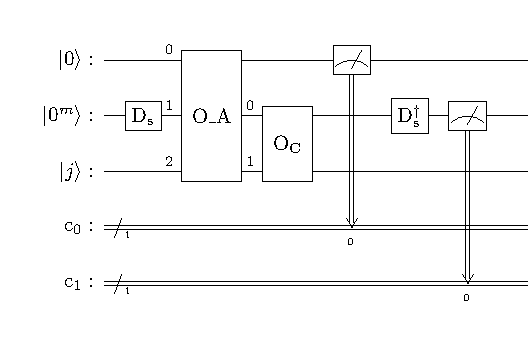
\includegraphics{pdf/main_circuit}
  \caption{
    A general schematic circuit drawing for the block encoding of an s-sparse matrix A
  }
  \label{fig:circuit2}
\end{figure}

\section{Instances of Block Encoding Circuits}\label{sec:instances}

In this section, we provide concrete instances showcasing the implementation of efficient $O_C$ and $O_A$ quantum circuits in theorem \ref{thm:main_result} tailored for structured sparse matrices.

\subsection{Block Encoding of Real Symmetric $2 \times 2$ Matrices}

As a concrete example, consider the real symmetric matrix:
\begin{equation}
  A =
  \begin{bmatrix}
    a & b \\
    b & a
  \end{bmatrix}.\label{eq:example_matrix}
\end{equation}
Although this matrix is dense, it can be treated as a $2$-sparse matrix with sparsity $s = 2$, since each row has at most two nonzero entries.

To construct its block encoding, we begin by defining the function $c(j, \ell)$, which determines the column index for a given row index $j$ and $\ell$-th nonzero entry. In this case, we can define:
\begin{equation}
  c(j,\ell) = (j + \ell) \mod 2,\label{eq:equation12}
\end{equation}
which allows us to implement the corresponding oracle $O_C$ using a single CNOT gate.

Next, consider the oracle $O_A$, which encodes the values of the nonzero entries. Since the entries $a$ and $b$ in~\eqref{eq:example_matrix} depend only on $\ell$, we can design a simple circuit that takes $\ket{\ell}$ as input and applies appropriate rotations. Specifically, we apply a rotation $R_y(\theta_1)$ when $\ell = 0$ and $R_y(\theta_2)$ when $\ell = 1$, where:
\begin{equation}
\theta_1 = 2\arccos(a), \quad \theta_2 = 2\arccos(b).
\end{equation}
Combining these two oracles, we obtain the full quantum circuit for the block encoding of matrix $A$. The resulting circuit is illustrated in Figure~\ref{fig:2x2_circuit}, where the control logic and rotation gates together realize an exact block encoding of the $2 \times 2$ symmetric matrix.

\begin{figure}[htbp]
  \centering
  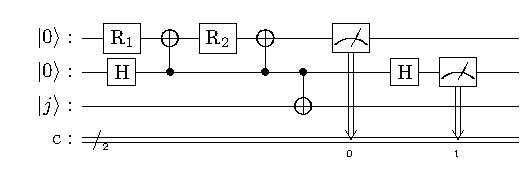
\includegraphics{pdf/2x2_circuit}
  \caption{Quantum circuit implementing the block encoding of a $2\times2$ real symmetric matrix.}
  \label{fig:2x2_circuit}
\end{figure}

\subsection{Block Encoding of Banded Circulant Matrices}\label{sec:banded_circulant}

Circulant matrices form a special class of structured matrices where each row is a cyclic shift of the preceding row. A \emph{banded circulant matrix} further restricts non-zero entries to a fixed bandwidth. Consider the following 2-banded circulant matrix with sparsity $s=3$:
$$
A =
\begin{bmatrix}
a & b & 0 & \cdots & 0 & c \\
c & a & b & \cdots & 0 & 0 \\
0 & c & a & \cdots & 0 & 0 \\
\vdots & \vdots & \vdots & \ddots & \vdots & \vdots \\
0 & 0 & 0 & \cdots & a & b \\
b & 0 & 0 & \cdots & c & a
\end{bmatrix}.\label{eq:example_circulant_matrix}
$$
For this matrix, the column mapping function $c(j, \ell)$ can be defined as:
$$
c(j, \ell) =
\begin{cases}
j-1 \ (\text{mod } N), & \ell = 0, \\
j, & \ell = 1 \text{ or } 3, \\
j+1 \ (\text{mod } N), & \ell = 2.
\end{cases}\label{eq:equation13}
$$

To implement the oracle $O_C$, observe that $j-1$ and $j+1$ correspond to cyclic permutation operations. These are represented by the left/right shift matrices $L$ and $R$:
$$
L =
\begin{bmatrix}
0 & 0 & \cdots & 0 & 1 \\
1 & 0 & \cdots & 0 & 0 \\
0 & 1 & \cdots & 0 & 0 \\
\vdots & \vdots & \ddots & \vdots & \vdots \\
0 & 0 & \cdots & 1 & 0
\end{bmatrix}, \quad
R =
\begin{bmatrix}
0 & 1 & 0 & \cdots & 0 \\
0 & 0 & 1 & \cdots & 0 \\
\vdots & \vdots & \vdots & \ddots & \vdots \\
0 & 0 & 0 & \cdots & 1 \\
1 & 0 & 0 & \cdots & 0
\end{bmatrix}.\label{eq:equation14}
$$

\begin{figure}[htbp]
  \centering
  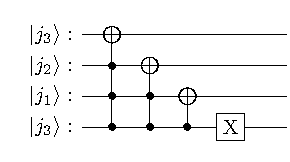
\includegraphics{pdf/circulant_l_shift} \quad
  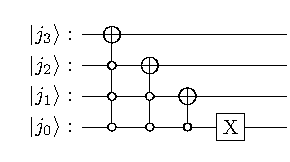
\includegraphics{pdf/circulant_r_shift}
  \caption{Quantum implementation of left-shift $L$ (left) and right-shift $R$ (right) using multi-qubit CNOT gates.}
  \label{fig:circulant_lr}
\end{figure}

The quantum circuits for $L$ and $R$ are shown in Figure~\ref{fig:circulant_lr}, which utilize controlled operations to realize cyclic shifts. Two qubits $\ket{\ell_1}$ and $\ket{\ell_2}$ are required to encode $\ell \in \{0,1,2,3\}$ according to Eq.~\eqref{eq:equation13}. The resulting oracle $O_C$ operates independently of $j$, leveraging the structure of $L$ and $R$.

For the amplitude oracle $O_A$, note that the matrix elements of $A$ depend only on $\ell$. Following the derivation in Section~\ref{sec:instances}, we construct a controlled rotation-based $O_A$ as shown in Figure~\ref{fig:circulant_oa}, with rotation angles:
$$
\theta_0 = 2\arccos(a-1), \quad
\theta_1 = 2\arccos(b), \quad
\theta_2 = 2\arccos(c).
$$

\begin{figure}[htbp]
  \centering
  \subfigure[Oracle $O_C$]{
    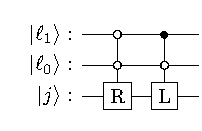
\includegraphics{pdf/circulant_oc}
    \label{fig:circulant_oc}
  }
  \subfigure[Oracle $O_A$]{
    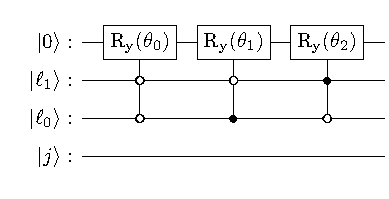
\includegraphics{pdf/circulant_oa}
    \label{fig:circulant_oa}
  }
  \subfigure[Alternative $O_A$ implementation]{
    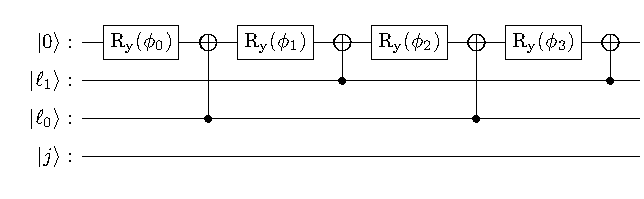
\includegraphics{pdf/circulant_oa2}
    \label{fig:circulant_oa2}
  }
  \caption{Oracles for banded circulant matrices. The alternative $O_A$ in (c) uses Walsh-Hadamard transformed phases $\phi_i$ for computational efficiency.}
\end{figure}

Figure~\ref{fig:circulant_oa2} presents an equivalent implementation of $O_A$ using a Walsh-Hadamard transformation to compute phase parameters $\phi_i$ from $\theta_i$. This formulation is particularly advantageous for digital implementations. Combining both oracles yields the complete block encoding circuit in Figure~\ref{fig:circulant_circuit}.

\begin{figure}[htbp]
  \centering
  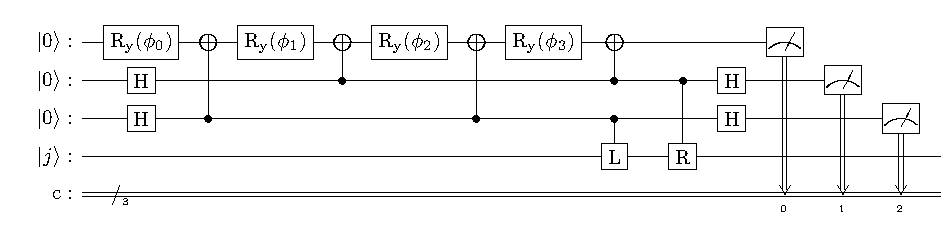
\includegraphics{pdf/circulant_circuit}
  \caption{Quantum circuit for block encoding banded circulant matrices.}
  \label{fig:circulant_circuit}
\end{figure}

The gate complexity analysis reveals:
- $\mathcal{O}(\log s)$ Hadamard gates, controlled rotations, and shift operators.
- Multi-qubit $L$/$R$ gates decompose into $\mathrm{poly}(n)$ two-qubit gates.
- No need to explicitly implement powers of shift operators (e.g., via repeated circuits), as shown in Lemma~\ref{lem:shift_optimization}.

Thus, the total gate count scales as $\mathcal{O}(n)$, maintaining efficiency for theoretical analysis and practical implementations.

\subsection{Block Encoding of an Extended Binary Tree}

The two preceding examples were relatively simple in structure, as the function $c(j, \ell)$ was straightforward to define and the matrix elements were fully determined by $\ell$. We now consider a more intricate example: the block encoding of an extended binary tree.

An extended binary tree can be represented by its adjacency matrix, which exhibits a sparse hierarchical structure. For an 8-node extended binary tree, the corresponding matrix is illustrated below:

\begin{figure}[htbp]
  \centering
  \begin{minipage}{0.35\textwidth}
    \centering
    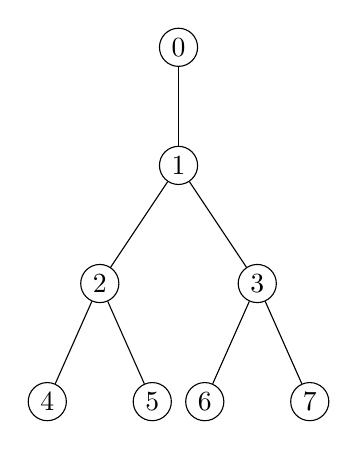
\begin{tikzpicture}[
        level/.style={sibling distance=40mm/#1},
        every node/.style={circle, draw, minimum size=1em, inner sep=2pt}
      ]
      \node {0}
      child {node {1}
        child {node {2}
          child {node {4}}
          child {node {5}}
        }
        child {node {3}
          child {node {6}}
          child {node {7}}
        }
      };
    \end{tikzpicture}
  \end{minipage}
  \hfill
  \begin{minipage}{0.6\textwidth}
    \centering
    \begin{equation}
      A =
      \begin{bmatrix}
        \gamma & \beta \\
        \beta & \alpha & \beta & \beta \\
        & \beta & \alpha & & \beta & \beta \\
        & \beta & & \alpha & & & \beta & \beta  \\
        & & \beta & & \gamma \\
        & & \beta & & & \gamma \\
        & & & \beta & & & \gamma \\
        &       & & \beta  & & &       & \gamma \\
      \end{bmatrix}.
    \end{equation}
  \end{minipage}
  \caption{Graph structure and adjacency matrix of an 8-node extended binary tree.}
  \label{fig:figure}
\end{figure}

In this matrix, $\gamma$ represents the self-loops at the root and leaf nodes, $\alpha$ corresponds to the internal nodes, and $\beta$ encodes the edge weights between connected nodes.

To construct the block encoding, we define $c(j, \ell)$ based on the tree's hierarchical structure. For a node $i$, its left and right children are indexed as $2i$ and $2i+1$, respectively. The column mapping function becomes:
\begin{equation}
  c(j, \ell) =
  \begin{cases}
    2j, & \text{if } \ell = 0 \text{ and } j < 2^{n-1},\\
    2j + 1, & \text{if } \ell = 1 \text{ and } j < 2^{n-1},\\
    j/2, & \text{if } \ell = 2 \text{ and } 2 \mid j,\\
    (j-1)/2, & \text{if } \ell = 3 \text{ and } 2 \nmid j,\\
    j, & \text{if } 4 \leq \ell \leq 7.
  \end{cases}\label{eq:equation17}
\end{equation}

Multiplication/division by 2 corresponds to left/right shift operations, which can be implemented via swap gates. For example, dividing $[0j_2j_1j_0]$ by 2 involves:
\begin{equation}
  [0j_2j_1j_0] 
  \xrightarrow{\text{swap}(j_0,j_1)} [0j_2j_0j_1] 
  \xrightarrow{\text{swap}(j_0,j_2)} [0j_0j_2j_1] 
  \xrightarrow{\text{swap}(j_0,0)} [j_00j_1j_2].
\end{equation}
Measurement on the first qubit may be required to ensure correctness. This procedure realizes an oracle mapping $\ket{0}$ to $\ket{j}$, denoted as $M_2$ and $D_2$. Combined with the control logic $L$ and $R$ from Eq.~\eqref{eq:equation14}, $O_C$ can be constructed as shown in Figure~\ref{fig:tree_oc}.

\begin{figure}[htbp]
  \centering
  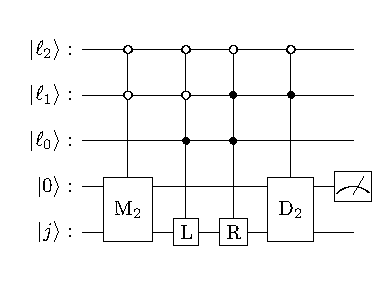
\includegraphics{pdf/tree_oc}
  \caption{Oracle $O_C$ implementation for binary tree matrices.}
  \label{fig:tree_oc}
\end{figure}

The $O_A$ oracle is constructed by analyzing the sparsity pattern. It can be expressed as a sequence of controlled rotations:
$$
\begin{aligned}
\theta_0 &= 2\arccos(\beta) \quad \text{for } \ell_2 = 0, \\
\theta_1 &= 2\arccos(\alpha/4) \quad \text{for } (\ell_2, j_2) = (1,0), \\
\theta_2 &= 2\arccos(\gamma/4) \quad \text{for } (\ell_2, j_2) = (1,1), \\
\theta_3 &= 2\arccos(\gamma/4 - \beta/2) - \theta_1 \quad \text{for } (\ell_2, j) = (1,0).
\end{aligned}
$$

By combining $O_C$ and $O_A$, we obtain the complete quantum circuit for the block encoding of the extended binary tree matrix (Figure~\ref{fig:tree_circuit}). This $8 \times 8$ implementation generalizes to larger matrices by adding qubits to the register.

\begin{figure}[htbp]
  \centering
  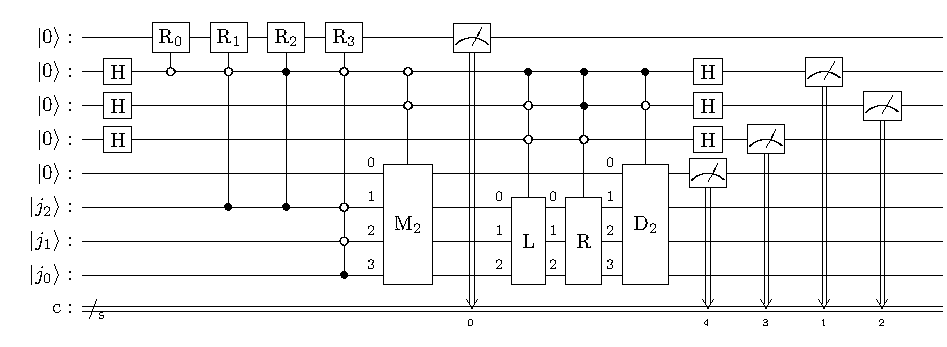
\includegraphics{pdf/tree_circuit}
  \caption{Complete quantum circuit for block encoding extended binary tree matrices.}
  \label{fig:tree_circuit}
\end{figure}

As discussed in Section~\ref{sec:block_encoding}, the gate count scales as $\mathcal{O}(\log s)$, and all operations decompose into $\mathrm{poly}(n)$ two-qubit gates. This demonstrates that the block encoding approach remains efficient even for complex hierarchical structures like extended binary trees.

\section{Efficient Block Encoding of Symmetric Stochastic Matrices without Scaling Factor}\label{sec:efficient-block-encoding-of-symmetric-stochastic-matrices-without-scaling-factor}
In the previous section, we introduced the general framework for constructing block encodings of $s$-sparse matrices in original paper.
However, this framework requires the scaling factor $1/s$ to ensure that the block encoding is exact.
In some situations, such as conducting quantum walks, we need to block encode symmetric stochastic matrices without the scaling factor.
In this section, we will explore how to construct block encodings of symmetric stochastic matrices without the scaling factor, which is a significant extension of the original framework.
Also we will use the quantum circuit to construct the block encoding of a quantum walk operator, which is a common application of symmetric stochastic matrices in quantum computing.

Before we proceed, we need to introduce the quantum singular value transformation (QSVT), which can be viewed as a powerful framework that allows quantum circuits to implement polynomial transformations of the singular values of a matrix embedded in a unitary operator.
The proof of Theorem~\ref{thm:qsp} and can be found in Gilyén et al.'s paper~\cite{Gilyen2019}.

\begin{theorem}[Quantum Signal Processing, QSP]
  \label{thm:qsp}
  Let
  \begin{equation}
    U(t) =
    \begin{bmatrix}
      t              & \sqrt{1 - t^2} \\
      \sqrt{1 - t^2} & -t
    \end{bmatrix}.\label{eq:equation15}
  \end{equation}
  There exists a set of phase angles $\Phi_d \equiv \{\phi_0, \ldots, \phi_d\} \in \mathbb{R}^{d+1}$ so that
  \begin{equation}
    U_{\Phi_d}(t) \equiv e^{i\phi_0 Z} \prod_{j=1}^d \left[ U(t) e^{i\phi_j Z} \right] =
    \begin{bmatrix}
      p(t)                 & -q(t)\sqrt{1 - t^2} \\
      q^*(t)\sqrt{1 - t^2} & p^*(t)
    \end{bmatrix},\label{eq:equation16}
  \end{equation}
  if and only if $p(t)$ and $q(t)$ are complex valued polynomials in $t$ and satisfy
  \begin{enumerate}
    \item $\deg(p) \leq d$, $\deg(q) \leq d - 1$;
    \item $p$ has parity $d \bmod 2$ and $q$ has parity $d - 1 \bmod 2$;
    \item $|p(t)|^2 + (1 - t^2)|q(t)|^2 = 1$, $\forall t \in [-1, 1]$.
  \end{enumerate}
  When $d = 0$, $\deg(q) \leq -1$ should be interpreted as $q = 0$.

\end{theorem}

In the theorem above, if we choose $\Phi_d \equiv (\phi_0, \phi_1, \ldots, \phi_d)$ as:
\begin{equation}
  \phi_j =
  \begin{cases}
    \pi/4, & j = 0 \text{ or } d \\
    \pi/2, & j = 1, \ldots, d-1,
  \end{cases}
\end{equation}
then $p(t)$ is the $d$th degree Chebyshev polynomial of the first kind.

For a polynomial $p(t)$ satisfying the conditions in Theorem~\ref{thm:qsp}, we can construct a quantum circuit that implements the polynomial transformation of the singular values of a matrix embedded in a unitary operator using QSP and quantization.

\begin{theorem}[Quantum Singular Value Transformation, QSVT]
  Consider d-degree polynomial $ P(x) $ satisfying QSP conditions,$U_A$ is a $(1,a,0)$-block-encoding of matrix $A$, we have:\\
  - For even $ d $:
  \begin{equation}
    e^{i\tilde{\phi}_0 Z_\Pi} \prod_{j=1}^{d/2} \left[ U_A^\dagger e^{i\tilde{\phi}_{2j-1} Z_\Pi} U_A e^{i\tilde{\phi}_{2j} Z_\Pi} \right] =
    \begin{pmatrix}
      P^\diamondsuit(A) & * \\
      *                 & *
    \end{pmatrix}
  \end{equation}

  - For odd $ d $:
  \begin{equation}
    e^{i\tilde{\phi}_0 Z_\Pi} U_A e^{i\tilde{\phi}_1 Z_\Pi} \prod_{j=1}^{(d-1)/2} \left[ U_A^\dagger e^{i\tilde{\phi}_{2j} Z_\Pi} U_A e^{i\tilde{\phi}_{2j+1} Z_\Pi} \right] =
    \begin{pmatrix}
      P^\vartriangleright(A) & * \\
      *                      & *
    \end{pmatrix}
  \end{equation}
  where $ \tilde{\phi}_j = \phi_j + (-1)^j \pi/2 $ , $\Pi = \ket{0}\bar{0}\otimes I$ and $ Z_\Pi = 2\Pi - I $.

  The equations above give a $(1,a+1,0)$-block-encoding of the matrix $P(A)$.
  The query complexity of $U_A$ is $d+1$.

  \label{thm:qsvt}
\end{theorem}

\section{Additional Tricks and Extensions on Block Encoding}

As established in Section~\ref{sec:block_encoding}, block encoding provides a systematic framework for representing sparse matrices in quantum circuits. Section~\ref{sec:instances} demonstrated concrete implementations for specific matrix structures. This section introduces advanced techniques that enhance the applicability of block encoding in both theoretical analysis and practical quantum algorithms.

\subsection{Hermitian Block Encoding}

While the general block encoding framework applies to arbitrary sparse matrices, it does not inherently preserve Hermiticity—a critical property in Hamiltonian simulation and quantum eigenvalue estimation. This subsection addresses this limitation by constructing Hermitian block encodings for sparse Hermitian matrices through Theorem~\ref{thm:main_result2}.

\begin{theorem}
  Suppose $A$ is a sparse Hermitian matrix of dimension $2^n$ with at most $s = 2^m$ non-zeros per column, with $m \leq n$. If a unitary $O_C$ satisfies
  \begin{equation}
    O_C \ket{\ell} \ket{j} = \ket{c(j, \ell)} \ket{j},\label{eq:equation18}
  \end{equation}
  where $c(j, \ell)$ is the row index of the $\ell$th non-zero element in the $j$th column, and if there exists a unitary $O_A$ such that
  \begin{equation}
    (I \otimes O_A) \ket{0} \ket{0} \ket{i} \ket{j} = \ket{0} \left( \sqrt{|A_{ij}|} \ket{0} + \sqrt{1 - |A_{ij}|} \ket{1} \right) \ket{i} \ket{j},
  \end{equation}
  for $A_{ij} = |A_{ij}| e^{i \theta_{ij}}$, where $\theta_{ij} \in [0, 2\pi)$, the square root is uniquely defined as $\sqrt{A_{ij}} = \sqrt{|A_{ij}|} e^{i \theta_{ij}/2}$. Then the unitary $U_A$ represented by the circuit shown in Fig.~\ref{fig:hermitian_encoding} is a Hermitian block encoding of $A$, where $D_s$ is a diffusion operator defined as
  \begin{equation}
    D_s \equiv I_2 \otimes \cdots \otimes
    \underbrace{H \otimes H \otimes \cdots \otimes H}_{m},
  \end{equation}
  and SWAP is a swap operator that swaps the last two $n$-qubit registers in Fig.~\ref{fig:hermitian_encoding} respectively.
  \label{thm:main_result2}
\end{theorem}

This construction leverages a key distinction in oracle design compared to Section~\ref{sec:block_encoding}: while Definition~\ref{eq:equation4} encodes $c(j, \ell)$ in the second register with $\ell$ preserved, Eq.~\ref{eq:equation18} maintains the column index $j$ in the second register while mapping $\ket{\ell}$ to $\ket{c(j, \ell)}$. The resulting circuit in Figure~\ref{fig:hermitian_encoding} ensures $U_A = U_A^\dagger$, thereby preserving the Hermitian structure of $A$.

\begin{figure}[htbp]
  \centering
  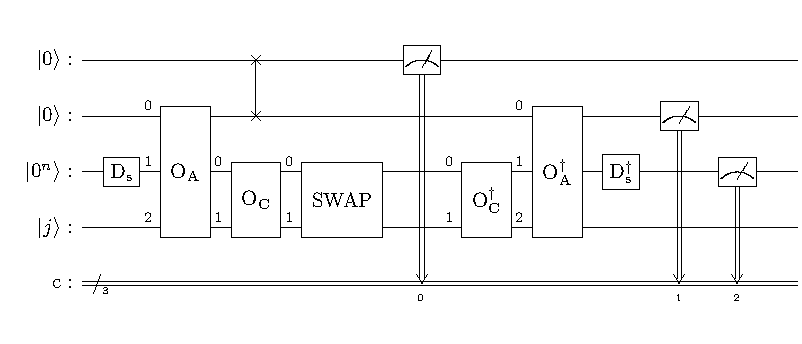
\includegraphics{pdf/hermitian_circuit}
  \caption{Quantum circuit for the Hermitian block encoding of a sparse Hermitian matrix $A$}
  \label{fig:hermitian_encoding}
\end{figure}

\subsection{Efficient Computation of Shift Matrix Powers}

Section~\ref{sec:banded_circulant} introduced cyclic shift operations for circulant matrices. We now present an optimized method to compute arbitrary powers of these shift operators—a common operation in block encoding algorithms.

For the left-shift matrix $L$ defined in Eq.~\eqref{eq:equation14}, observe the recursive decomposition:
\begin{equation}
L_n^2 = L_{n-1} \oplus I_2.\label{eq:equation19}
\end{equation}
This identity enables a binary exponentiation approach similar to classical fast exponentiation algorithms. Given a binary-encoded exponent:
\begin{equation}
j = [j_{n-1} j_{n-2} \cdots j_1 j_0] = \sum_{i=0}^{n-1} j_i 2^i,
\end{equation}
we can decompose the power operation as:
\begin{equation}
L_n^j = \prod_{i=0}^{n-1} \left(L_n^{2^i} \right)^{j_i}.
\end{equation}
Applying Eq.~\ref{eq:equation19} recursively yields:
\begin{equation}
L_n^{2^i} = L_{n-i} \oplus \underbrace{I_2 \oplus \cdots \oplus I_2}_{i}.
\end{equation}
This hierarchical structure allows implementation of $L_n^j$ in $\mathcal{O}(n)$ time using controlled unitaries $O_1, O_2, \ldots, O_{n-1}$. Figure~\ref{fig:shift_power} illustrates this construction for $n=3$.

\begin{figure}[htbp]
  \centering
  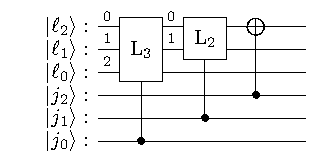
\includegraphics{pdf/shift_power}
  \caption{Circuit implementing $L_n^j$ for $n=3$}
  \label{fig:shift_power}
\end{figure}

\subsection{Quantum Walks and Block Encoded Discriminant Matrices}

We explores the interplay between quantum walks, block encodings, and classical Markov chains, highlighting how block encoding techniques enhance the efficiency of quantum algorithms for graph problems. This subsection summarizes the key theoretical insights and practical implications.

\subsubsection{Properties of Markov Chain Matrices}
A classical Markov chain is governed by a stochastic matrix $ P $, where $ P_{ij} $ represents the transition probability from state $ i $ to $ j $. The stationary distribution $ \pi $ satisfies $ \pi^\top P = \pi^\top $, and for an ergodic chain (irreducible and aperiodic), $ \pi $ is unique. A reversible Markov chain further satisfies the detailed balance condition $ \pi_i P_{ij} = \pi_j P_{ji} $, enabling the construction of a symmetric discriminant matrix $ D $ with entries:
\begin{equation}
D_{ij} = \sqrt{P_{ij} P_{ji}}. \label{eq:discriminant_matrix}
\end{equation}
This matrix $ D $ shares eigenvalues with $ P $, and its symmetric structure simplifies spectral analysis. The stationary state $ \ket{\pi} = \sum_i \sqrt{\pi_i} \ket{i} $ becomes the principal eigenvector of $ D $, satisfying $ D \ket{\pi} = \ket{\pi} $.

\subsubsection{Szegedy Quantum Walk as a Block Encoding}
The Szegedy quantum walk generalizes classical random walks by leveraging block encodings of $ D $. Given a reversible $ P $, the walk operator $ U_Z $ is constructed via two reflection operators $ R_{\Pi_1} $ and $ R_{\Pi_2} $, defined as:
\begin{equation}
U_Z = R_{\Pi_2} R_{\Pi_1}, \quad \text{where } R_{\Pi_l} = 2 \sum_j \ket{\psi_l^j}\bra{\psi_l^j} - I.
\end{equation}
Here, $ \ket{\psi_1^j} $ and $ \ket{\psi_2^j} $ are quantum states encoding rows/columns of $ \sqrt{P} $. Crucially, $ U_Z $ corresponds to a block encoding of $ T_2(D) $, where $ T_k $ denotes the Chebyshev polynomial of degree $ k $. More generally, $ k $-step Szegedy walks implement $ T_{2k}(D) $, enabling polynomial transformations of $ D $'s spectrum.

\subsubsection{Quantum Speedup in Detecting Marked Vertices}
The section demonstrates a quadratic speedup in detecting a marked vertex in a graph using quantum walks. Consider a complete graph $ G $ with $ N $ vertices:

For classical setting, a random walk with transition matrix $ P $ requires $ \mathcal{O}(N) $ steps to identify a marked vertex due to the spectral gap $ \delta = \mathcal{O}(1/N) $; For quantum setting, by block encoding $ D $ and applying $ U_Z^k $, the success probability of measuring $ \ket{0^n} $ drops to $ \mathcal{O}(1/N) $ after $ k = \mathcal{O}(\sqrt{N}) $ steps. This follows from the Chebyshev polynomial amplification:
\begin{equation}
T_k(1 - \delta) \approx \cos\left(k \sqrt{2\delta}\right), \quad \text{yielding } p(\ket{0^n}) = \frac{1}{N} + \left(1 - \frac{1}{N}\right) T_k^2(1 - \delta).
\end{equation}
When $ k \propto \sqrt{N} $, the interference effect sharply distinguishes the marked state, achieving a quadratic speedup over classical methods.

\subsubsection{Implications and Experimental Validation}

This analysis underscores some key advantages of block encoding in quantum walks:

\begin{enumerate}
  \item Spectral Amplification: Chebyshev polynomials $ T_k(D) $ amplify eigenvalue separations, accelerating convergence to stationary states.
  \item Efficient Implementation: Block encoding allows direct manipulation of $ D $ without explicit matrix exponentiation, enabling efficient quantum circuits for large graphs.
  \item Quadratic Speedup: The quantum walk framework achieves a quadratic speedup in detecting marked vertices, surpassing classical random walks.
\end{enumerate}

In experiment, for $ n = 6 $ qubits, block-encoded discriminant matrices for both marked and unmarked graphs are constructed. Repeated application of the quantum walk operator confirms that the success probability collapses at $ k \propto \sqrt{N} $, aligning with theoretical predictions.

These results position block encoding as a foundational tool for translating classical probabilistic algorithms into quantum-accelerated counterparts, particularly in graph theory and search problems.

\bibliographystyle{unsrt}
\bibliography{references}
\end{document}